\chapter[Delayed Bifurcation]{Delayed Bifurcation}

Consider a bistable system with operating characteristics as shown in Fig. \ref{fig:strogatz-wk21}. 
\begin{figure}[!h]
	\centering
	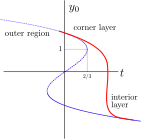
\includegraphics[width=0.5\textwidth]{./plots/pdf/delayed-bifurcation.pdf}
	\caption{The solid/dashed blue curves show the stable/unstable points. As the control parameter $r$ is varied infinitesimally slowly, the translucent ``hysteresis'' curve is traced. For a non-zero sweep-rate shown in red, a \emph{delayed bifurcation} is seen.}
	\label{fig:strogatz-wk21}
\end{figure}\\
How does the ``delay'' depend on the sweep-rate of the control parameter? Here the sweep-rate is taken to be small which lets us perform asymptotic analysis. We will show that the delay $\propto \epsilon^{2/3}$ where $\epsilon$ is the rate of sweeping ($\epsilon \rightarrow 0^+$). Methods from the Boundary Layer theory and Airy's functions will be used. \\
\ \newline
The curve in Fig. \ref{fig:strogatz-wk21} is sketched using a functional form $f(y) = y^3/3-y$. To introduce a time-dependence to our model, we may write
\begin{gather*}
	\frac{\md y}{\md \tau} = y - \frac{y^3}{3} - \epsilon \tau
\end{gather*}
where our control parameter $r=\epsilon \tau$ varies slowly through the introduction of $\epsilon$. Let us first understand the phase-portrait when $\epsilon=0$ (Fig. \ref{fig:strogatz-wk21-model}). It is worth noting that the \emph{fixed points} occur when $\md y/\md \tau=0$, i.e. 
\begin{gather*}
	y=0 \qquad y = \pm \sqrt{3}
\end{gather*}
Note that when $f(y)>0$, $y'>0$, so $y$ increases and the particle is pushed towards the right (etc.), ergo, the \emph{stable} fixed points are $y=\pm \sqrt{3}$. The max/min occur at $f'(y)=0$, i.e.
\begin{gather*}
	y = \pm 1 \qquad \implies f(y) = \pm \frac{2}{3}
\end{gather*}
Now if the parameter $r(\tau)$ is slowly varying, this is simply the intercept (constant). The stable and unstable points are seen to come together and eventually coalesce. Eventually, we are left with only one stable point. Therefore, a system which would have started at a large value ($>O(1)$), moves towards the stable point $y=\sqrt{3}$, but as the stable point moves downwards due to $r(\tau)$, it jumps all the way to $y \sim -\sqrt{3}$.
\begin{figure}[!h]
	\centering
	\includegraphics[width=0.75\textwidth]{./plots/pdf/strogatz-wk21.pdf}
	\caption{Here $r(\tau)=0.5$. The stable fixed points are shown in pink and the unstable fixed point is shown in blue.}
	\label{fig:strogatz-wk21-model}
\end{figure}\\
Observe that since $f(y)=2/3$, we expect the ``jump'' when $\epsilon \tau \approx 2/3$ (the curve needs to lower by this amount for the stable/unstable points to coalesce). We proceed to analyze this more closely using asymptotics. \\
\ \newline
Let $t=\epsilon \tau$, which transforms our ODE to
\begin{gather}
	\epsilon \frac{\md y}{\md t} = y - \frac{y^3}{3} - t \label{eqn:wk21-ode}
\end{gather}
We can see immediately that the \underline{outer} solution is when $\epsilon=0$. With the ansatz
\begin{gather*}
	y = y_0 + \epsilon y_1 + \dots
\end{gather*}
at $O(\epsilon^0)$ we have a simple algebraic equation
\begin{gather}
	y_0 - \frac{y_0^3}{3} = t \label{eqn:wk21-outer}
\end{gather}
From Fig. \ref{fig:strogatz-wk21}, we see that the sytem has a corner layer and an interior layer. We start at the upper branch where $y_0 >1$. Recall that the jump occurs at $y_0=1$ which corresponds to $t=2/3$.
\begin{figure}[!h]
	\centering
	\includegraphics[height=0.4\textwidth]{./plots/pdf/strogatz-wk21-layers.pdf}
	\includegraphics[height=0.4\textwidth]{./plots/pdf/delayed-bifurcation-layers.pdf}
	\caption{(Left) Plot of eqn. \ref{eqn:wk21-outer}. (Right) The various regions in the language of asymptotics.}
	\label{fig:delayed-bifurcation-layers}
\end{figure} \\\\
\underline{Corner layer:} Use ``tilde'' to denote corner variables. We look near $t \approx 2/3$ and $y \approx 1$. Define 
\begin{equation}\label{eqn:wk21-corner-sub}
\begin{gathered}
\tilde{t} = \frac{t-2/3}{\epsilon^\alpha} \\ y(t) = \tilde{Y}(\tilde{t}) = 1 + \epsilon^\gamma \tilde{Y}_1 + \epsilon^{2\gamma} \tilde{Y}_2 + O(\epsilon^{3\gamma})
\end{gathered} 
\end{equation}
In terms of our new variables, eqn. \ref{eqn:wk21-ode} reads\footnote{Using $(a+b+c)^3 = a^3 + b^3 + c^3 + 3a^2b + 3 ab^2 + 3ac^2 + 3a^2c + 3bc^2 + 3b^2c$}
\begin{align*}
 \frac{\epsilon}{\epsilon^\alpha}\frac{\md }{\md \tilde{t}} \left(\epsilon^\gamma \tilde{Y}_1 + \epsilon^{2\gamma}\tilde{Y}_2 + \dots\right) &= \left(1 + \epsilon^\gamma \tilde{Y}_1 + \epsilon^{2\gamma} \tilde{Y}_2 + \dots \right)\\
 &- \frac{1}{3}\left(1 + \epsilon^\gamma \tilde{Y}_1 + \epsilon^{2\gamma} \tilde{Y}_2 + \dots \right)^3 \\
 &- \left[\frac{2}{3} + \epsilon^\alpha \tilde{t} \right] \\
 \epsilon^{1-\alpha + \gamma} \frac{\md}{\md \tilde{t}} \left(\tilde{Y}_1 + \epsilon^\gamma \tilde{Y}_2 + \dots\right) &= \left(\cancel{1 - \frac{1}{3} - \frac{2}{3}}\right) - \epsilon^\alpha \tilde{t} \\
 &+ \left(\cancel{\epsilon^\gamma \tilde{Y}_1} + \cancel{\epsilon^{2\gamma} \tilde{Y}_2}\right) \\
 &-\frac{1}{3} \left( 3 \cancel{\epsilon^\gamma \tilde{Y}_1} + 3 \epsilon^{2\gamma}\tilde{Y}^2_1 + 3 \cancel{\epsilon^{2\gamma} \tilde{Y}_2} \right) + O(\epsilon^{3\gamma})\\
 &= -\epsilon^\alpha \tilde{t} - \epsilon^{2\gamma}\tilde{Y}_1^2 + O(\epsilon^{3\gamma})
\end{align*}
A three-term dominant balance arises when (no evolution equation for $\tilde{Y}_2$)
\begin{gather*}
	1 - \alpha + \gamma = 2\gamma = \alpha 
\end{gather*}
This yields
\begin{gather}
	\gamma = \frac{1}{3} \qquad \alpha = \frac{2}{3} \label{eqn:wk21-corner-scaling}
\end{gather}
which already indicates that the corner layer width
\begin{gather*}
	\Delta t \propto \epsilon^{2/3}
\end{gather*}
Also note that the neglected terms of $O(\epsilon^{3\gamma}) = O(\epsilon) \ll \epsilon^{2/3}$. With this choice of $\alpha$ and $\gamma$, our ODE in the corner layer reads
\begin{gather}
	\frac{\md \tilde{Y}_1}{\md \tilde{t}} = - \tilde{Y}^2_1 - \tilde{t} \label{eqn:wk21-corner-nonlin-ode}
\end{gather}
This is the famous ``Riccati equation'' and is solved with the neat substitution
\begin{gather}
	\tilde{Y}_1 = \frac{W'}{W} \label{eqn:wk21-riccati-sub}
\end{gather} 
Our corner layer eqn. now reads
\begin{gather}
	W'' = -\tilde{t} W \label{eqn:wk21-airy}
\end{gather}
This is the Airy's equation (except with $-\tilde{t}$ instead of $\tilde{t}$). Also note that our nonlinear ODE (eqn. \ref{eqn:wk21-corner-nonlin-ode}) has been transformed into a linear ODE (eqn. \ref{eqn:wk21-airy}) through the clever transform (eqn. \ref{eqn:wk21-riccati-sub}). The solution to eqn. \ref{eqn:wk21-airy} is simply
\begin{gather*}
	W(\tilde{t}) = a_0 \mathrm{Ai}(-\tilde{t}) + a_1 \mathrm{Bi}(-\tilde{t})
\end{gather*}
The corner solution at the lowest order is then
\begin{gather*}
	\tilde{Y}_1 = \frac{-[a_0 \mathrm{Ai}'(-\tilde{t}) + a_1 \mathrm{Bi}'(-\tilde{t})]}{a_0 \mathrm{Ai}(-\tilde{t}) + a_1 \mathrm{Bi}(-\tilde{t})}
\end{gather*}
Next, we determine $a_0$ and $a_1$ to match this to the outer solution. From Fig. \ref{fig:delayed-bifurcation-layers} note that for the outer solution $t<2/3$ everywhere; therefore we want to approach $2/3$ from the negative side, i.e. $t \rightarrow 2/3^-$, so with respect to the new variable $\tilde{t} \rightarrow -\infty$. Also note that $y_0 >1$ and $y$ comes down from above. \\
\ \newline
From intuition, since Bi($\infty$) tends to blow up, we expect $a_1=0$. But this can we worked out more systematically.  \\ 
\ \newline
It is worth noting the following asymptotic behavior {\color{red}[in Mathematica notebook by Prof. Strogatz.]}
\begin{align*}
	\lim\limits_{\tilde{t} \rightarrow -\infty} \left[-\frac{\mathrm{Ai}'(-\tilde{t})}{\mathrm{Ai}(-\tilde{t})}\right] &=+ \sqrt{-\tilde{t}} \\
	\lim\limits_{\tilde{t} \rightarrow -\infty} \left[-\frac{\mathrm{Bi}'(-\tilde{t})}{\mathrm{Bi}(-\tilde{t})}\right] &=- \sqrt{-\tilde{t}}
\end{align*}
To match in the corner layer, we find the asymptotics of the outer solution for $t\rightarrow 2/3^-$ and $y_0 \rightarrow 1^+$. From eqns. \ref{eqn:wk21-outer}, \ref{eqn:wk21-corner-sub} and \ref{eqn:wk21-corner-scaling}
\begin{align*}
	\left(1 + \epsilon^{1/3} \tilde{Y}_1 + \dots \right) - \frac{1}{3}\left(1 + \epsilon^{1/3} \tilde{Y}_1 + \dots\right)^3 = \frac{2}{3} + \epsilon^{2/3} \tilde{t}
\end{align*}
Comparing powers
\begin{align*}
	-\frac{\tilde{Y}_1^3}{3} = 0 \qquad 
	 \tilde{Y}_1=\pm \sqrt{-\tilde{t}}
\end{align*}
Since we know $y_0>1$ on the upper branch, we pick the positive non-zero root. This also implies that we are interested in the [$-\mathrm{Ai}'(-\tilde{t})/\mathrm{Ai}(-\tilde{t}$)] solution which asymptotes to $+\sqrt{-\tilde{t}}$ and discard the Bi terms by setting $a_1=0$.
\begin{align*}
	y_0 &\sim 1 - \epsilon^{1/3} \frac{\mathrm{Ai}'(-\tilde{t})}{\mathrm{Ai}(-\tilde{t})} \\
	&\sim 1 + \epsilon^{1/3} \sqrt{-\tilde{t}}
\end{align*}
Now
\begin{align*}
t &= \frac{2}{3} + \epsilon^{2/3} \tilde{t} \\
&=\frac{2}{3} + \underbrace{\epsilon^{2/3} (2.338\dots )}_\text{delay} 
\end{align*}
since $\tilde{t}=2.338\dots $ is the point when the function is `falling off a cliff'.
\begin{figure}[!h]
	\centering
	\includegraphics[width=0.65\textwidth]{./plots/pdf/strogatz-wk21-aip_ai.pdf}
	\caption{The quantity [$-\mathrm{Ai}'(-\tilde{t})/\mathrm{Ai}(-\tilde{t}$)] blows up when Ai crosses its zeros.}
	\label{fig:strogatz-wk21-aip_ai}
\end{figure}\\
\underline{Interior layer:} From Fig. \ref{fig:strogatz-wk21-aip_ai} it is clear that the corner layer solution $y_0 \rightarrow -\infty$ and a third \emph{interior layer} is therefore needed to match onto the lower branch in Fig. \ref{fig:delayed-bifurcation-layers}. In this region we look in the neighborhood of $t>t_0$:
\begin{align*}
	t^\ast = \frac{t-t_0}{\epsilon^\kappa} \qquad t_0 = \frac{2}{3} + \epsilon^{2/3}\tilde{t}_0 \\
	y(t) = Y^\ast (t^\ast) \sim Y_0^\ast (t^\ast ) + \dots 
\end{align*}
The jump is $O(1)$. Our governing ODE becomes
\begin{gather}
\epsilon^{1-\kappa} \frac{\md Y_0\ast}{\md t^\ast } = Y_0^\ast - \frac{Y_0^\ast}{3} - \left[\epsilon^\kappa t^\ast + \frac{2}{3} + \epsilon^{2/3}\tilde{t}_0\right]
\end{gather}
The $Y_0^\ast$ terms can only balance on both sides when $\kappa =1$ (usual scaling in layer: time-scale $O(\epsilon)$). 
\begin{gather}
	\frac{\md Y_0\ast}{\md t^\ast } = Y_0^\ast - \frac{Y_0^\ast}{3} - \frac{2}{3} \label{eqn:wk21-interior-ode}
\end{gather}
\begin{figure}[!h]
	\centering
	\includegraphics[width=0.65\textwidth]{./plots/pdf/strogatz-wk21-interior.pdf}
	\caption{Plot of eqn. \ref{eqn:wk21-interior-ode}. The left fixed point is stable whereas the right fixed point is half-stable.}
	\label{fig:strogatz-wk21-interior}
\end{figure}\\
Now after we have gone around the corner, $Y_0^\ast<1$; this is our initial condition, which then implies that we end up at the left stable fixed point.












